%\subsection{Pedagogical development}

%The first section describes "How do you get people to learn things?", cognitive psychology. Often school is studied, where learning is about being taught a subject, and then to pass a test. E-learning tools are often designed to do similar things to what schools does.

%The second section describes "How do you get people to behave differently?", social psychology. One area of research is about building habits. This is highly relevant in e-learning, where behavior change may be necessary to build the habit of using an app or a digital tool repeatedly.

%\include{theory/learning/pedagogical-development/cognitive_psychology}

%\subsubsubsection{Learning}

  \subsubsection{Learning Entrepreneurship: Mapping Educational Objectives with Bloom's Revised Taxonomy}

  What to teach should be determined by the learning objectives of the activity.

  Learning activities often involve both lower order and higher order thinking skills as well as a mix of concrete and abstract knowledge. This needs to be designed for \todo{Konrad: specify}. Here, Bloom's revised taxonomy can provide usable insight into how to design, by the combination between lower or higher cognitive complexity, and concrete (factual or conceptual) or abstract knowledge (procedural or metacognitive). \citep{cheong} The taxonomy thus provides a framework for determining and clarifying learning objectives. See figure \ref{fig:revised-bloom} from \citep{heer}. Each colored block is an example of a learning objective matching with the two dimensions. The figure also explains the different concepts. Depending on the objective, it fits differently into the Knowledge dimension and Cognitive Process dimension of Bloom's Revised Taxonomy. \citep{krathwohl}

  \begin{figure}[h]
    \centering
    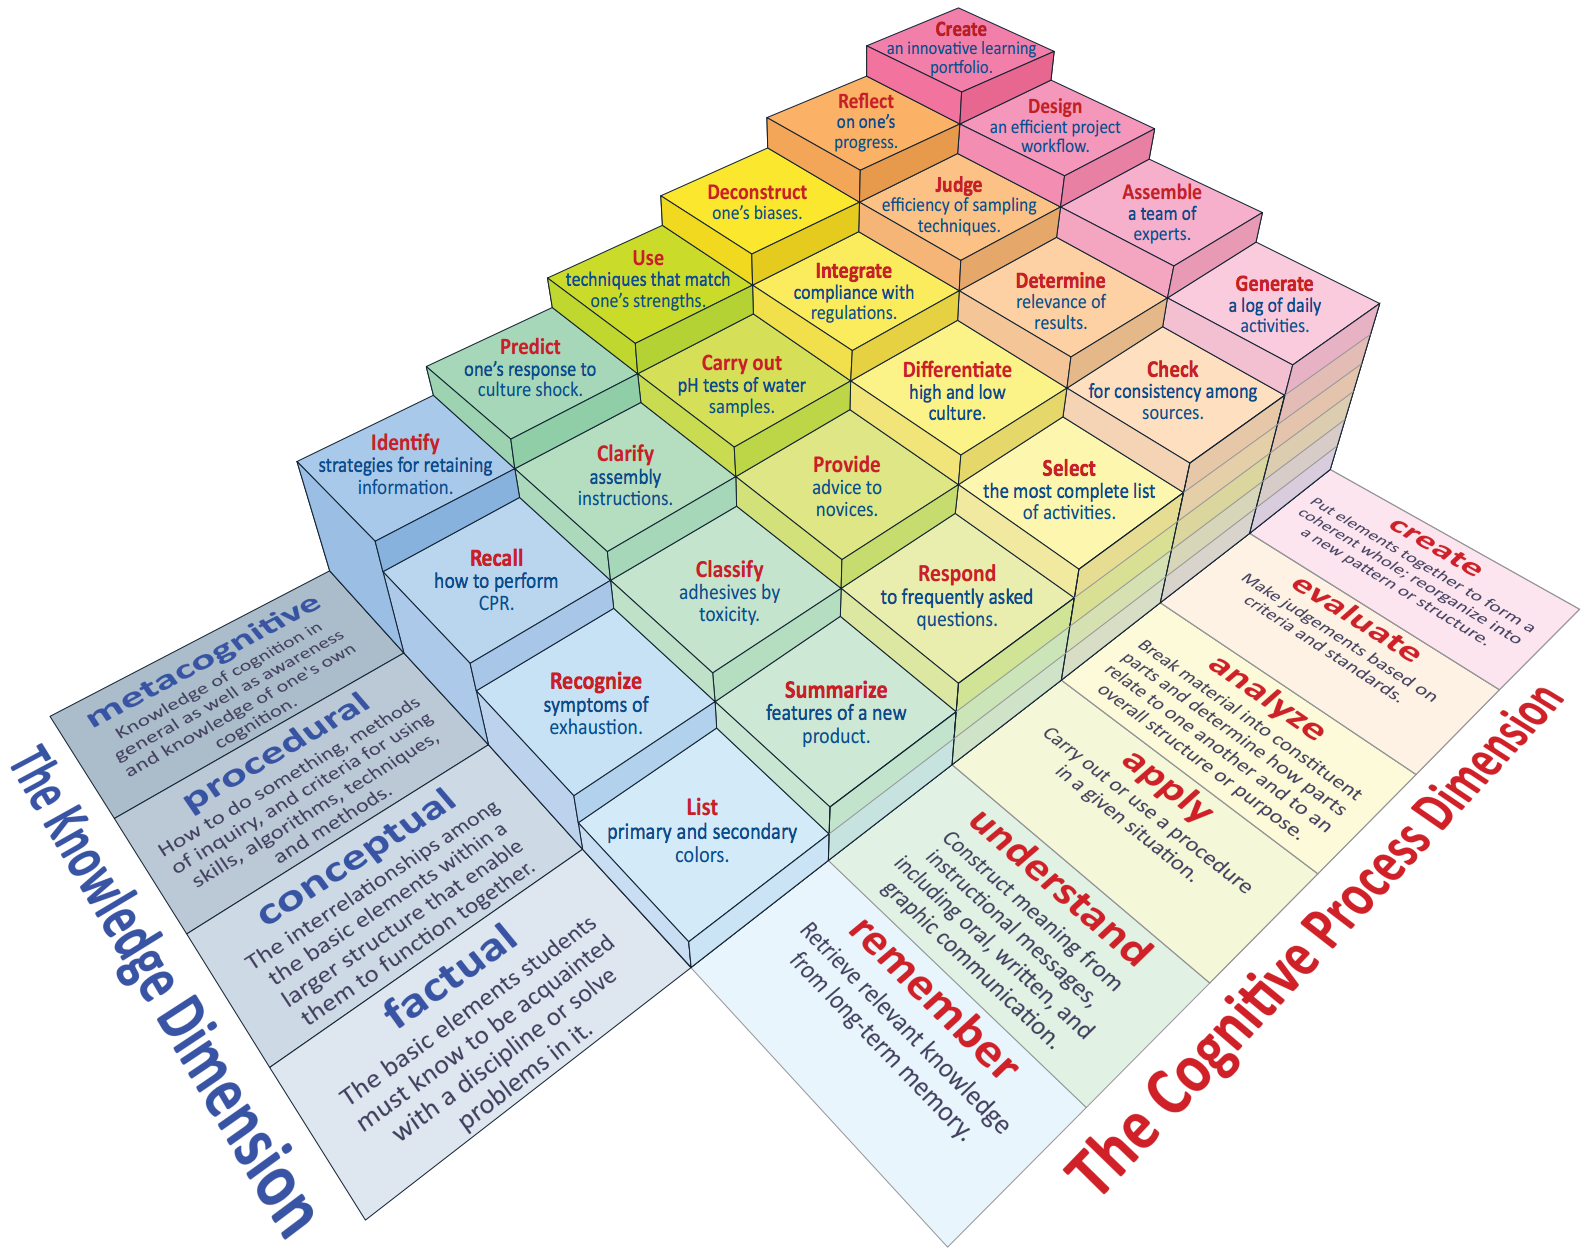
\includegraphics[width=1.0\textwidth]{RevisedBloom.png}
    \caption{Bloom's revised taxonomy visualised with examples of different learning objectives.}
    \label{fig:revised-bloom}
\end{figure}

  Bloom's revised taxonomy can be useful both to map learning objectives for entrepreneurship and as an entrepreneurship coach. To craft good multiple-choice questions could be an art, but to map the question to the learning objective makes it into more of a science:

  Entrepreneurship topic question: "What is financial literacy?" (= \textit{conceptual} and \textit{remember})

  To simulate a procedural environment, the question can be presented as a scenario:

  Entrepreneurship coach question: "It turns out that 10 youth have not carried out the business action, what should you do?" (= metacognitive and evaluating)

  There are several traps that the person formulating the question and answer alternatives can fall into, in the case of multiple-choice, where a good question might be de-amplified because of the answer alternatives.

  Consider the coach being asked to give business advice to a fictional youth named Adam: "Adam wants to start a business that is based on a product. which business should he start?". Before, the coach has been given questions on what a service and product is (factual remember), what the difference is (factual understand), and been given examples (conceptual analyze). Now, the skills are being put to a procedural test.

  If the answer alternatives are obvious (or memorized), the learning will be lower than scoring high on Bloom's revised taxonomy.

  If the answers are high-quality alternatives, all of the answers must be evaluated and considered. In such cases, multiple-choice learning can actually amplify learning, via \textit{learning by repetition} or \textit{learning by thinking}.

  In this case 3-4 valid alternatives might be: "Start a salon", "Start selling soap", "Start a bricklaying business".

  It is still hard to score high on the knowledge and cognitive dimension using techniques such as multiple-choice with entrepreneurship and coaching. This is however necessary, if the app should reach the learning objectives of YoungDrive.

  There may need to be additions to the multiple-choice design, and not only content. Such design ideas may be utilizing flip card techniques (don't see answer alternatives until you've thought of your answer), or asking "How sure are you?", both encouraging metacognitive thinking.

  More ambitious ideas, would be to simulate the entrepreneur coach environment more accurately than via text (using more channels, like audio, video, voice), or to do simulations instead of using multiple-choice. The advantage of multiple-choice, is that data can be collected easily, and that it serves the target group of first-time smartphone users, and because of ease of implementation.

  \subsubsection{Building skills: by Spaced practice, Deliberate practice and Perceptual exposure}

  Spaced practice deals with spreading out learning, with the purpose of not forgetting. E.g. Clark \citep{gates} concludes that spaced learning versus massed learning (no rest between sessions) did have a memory benefit in their study.

  Taking spaced learning into consideration, could mean making the user apparent on the person's meta-cognitive ability (your personal insight of what you'll remember and when you are likely to forget), and meta-memory (when you need to repeat information in order not to forget).

  Clark \citep{gates} found no evidence of consistent correlation between total duration and effects on learning outcomes in their study. So how do you design for optimal learning outcomes of skills, particularly if those are entrepreneurial or coaching skills?

  When building skills, Sierra suggests deliberate practice \citep{yengin} \citep{sierra}. The goal is to help users practice right, by designing practice exercises that will take a fine-grained task from unreliable to 95\% reliability, within one to three 45-90-minute sessions.

  Deliberate practice has been proven to be an effective way to build skills. It has also been tested before for mobile learning environments. \citep{yengin}

  Sierra \citep{sierra} suggests skills to be divided into three buckets: can't do (but need to do), can do with effort, and mastered (reliable/automatic). The goal then is to move skills from can't do into mastered, in the best way possible. See figure \ref{fig:sierra-practice} from Sierra \citep{sierra}. Sierra says, if you can’t get the user to 95\% reliability within this time, stop trying; you need to redesign the sub-skill. \citep{sierra}

  \begin{figure}[h]
    \centering
    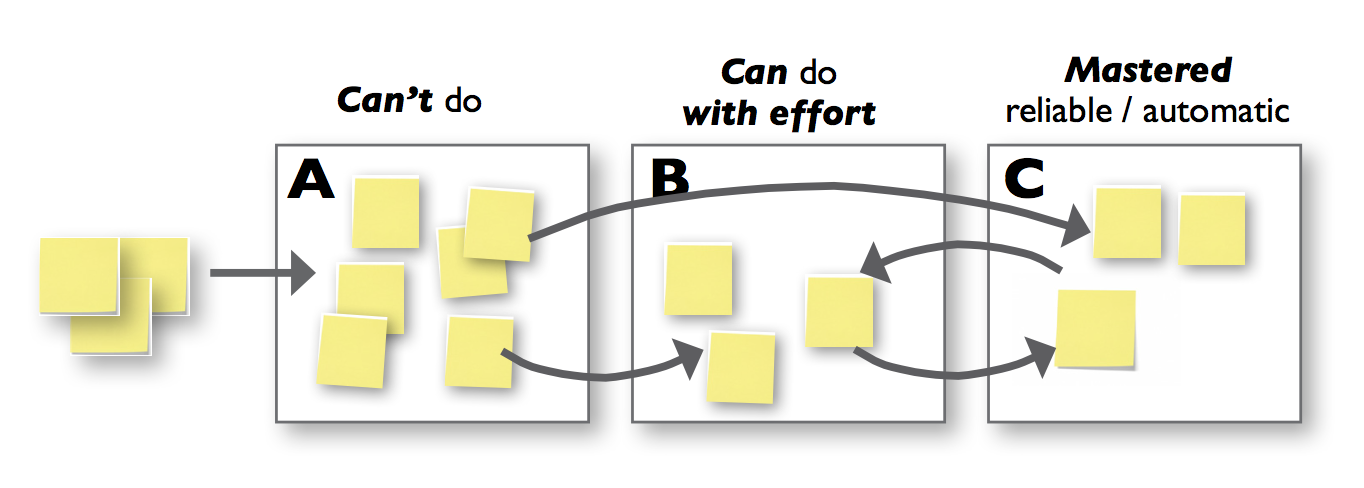
\includegraphics[width=0.8\textwidth]{SierraPractice.png}
    \caption{Moving skills from A (Can't do) to B (Can do with effort) into C (Mastered) can move different ways, depending on how effective the learning is. Deliberate practices focuses on A-B-C, while perceptual expose enables A to C. Reflection allows knowledge to go backwards, to get better at the skill than previously possible. An example might be to teach "Financial literacy". Concepts and factual knowledge (like what income and profit is) might need to move A-B-C, whereas entrepreneurship skills (like taking financial decisions) can move A-C if it becomes intuitive for the user, e.g. via having been exposed to a lot of trial-and-error examples in the app.}
    \label{fig:sierra-practice}
  \end{figure}

  Desirable difficulties applies here, meaning that during deliberate practice, it may feel as if learning gets more and more difficult, but in the long term the user is actually learning more. As a result, less people does true deliberate practice, but they do not get the same reward in return. This needs to be designed for, e.g. using social psychology\todo{Konrad: how?}.

  By deliberate practice, you can practice better. The second attribute of those who became experts, were that they were exposed to high quality, high quantity examples of expertise. \citep{sierra}

  It shows that whenever a skill relies on intuition, we could try exposing the user a well-designed trail and error test. In the case of multiple-choice questions, this could be done by exposing users to very high-quality samples during a very limited time. Perceptual knowledge includes teaching what we think of as expert intuition (like being a good entrepreneurship coach).

  Sierra shows how researchers have repeatedly, by well designed tests, been able to quickly build expertise by trial-and-error feedback. A novice would hazard a guess and an expert would say yes or no. Eventually the novices became, like their mentors, masters of the expertise that could otherwise would have been intangible for long.

  \subsubsection{Learning from Assessment}\label{learning-assessment}

  Knowing what learners know, and don't know, is crucial to effective learning, Luckin \citep{luckin} says.

  Assessment can partly help to design for flow, matching challenge and ability \citep{bruhlmann}, which is effective for intrinsic motivation (see next chapter).

  Moreover, it also has cognitive benefits. It can help to offer appropiate feedback, increase learners' awareness of their learning needs, and give accurate assessment and analysis, and allows learning to be tailored.

  By recognizing differences of students, in their ability to understand what they know and how they can progress, it is possible to ensure that everyone achieves their full potential.

  Effective assessment by a teacher or agent includes individual feedback (task-oriented and informal) and appropiate feed-forward advice. Sitzmann \cite{sitzmann} has studied how questions used to prompt self-monitoring and self-evaluation benefit learning, showing gradual, positive effect on learning. Regarding multiple-choice tests, Nicol \cite{nicol} gives seven principles of good feedback practice, see figure \ref{figure:multiple-choice}.

  \begin{figure}[h]
    \centering
    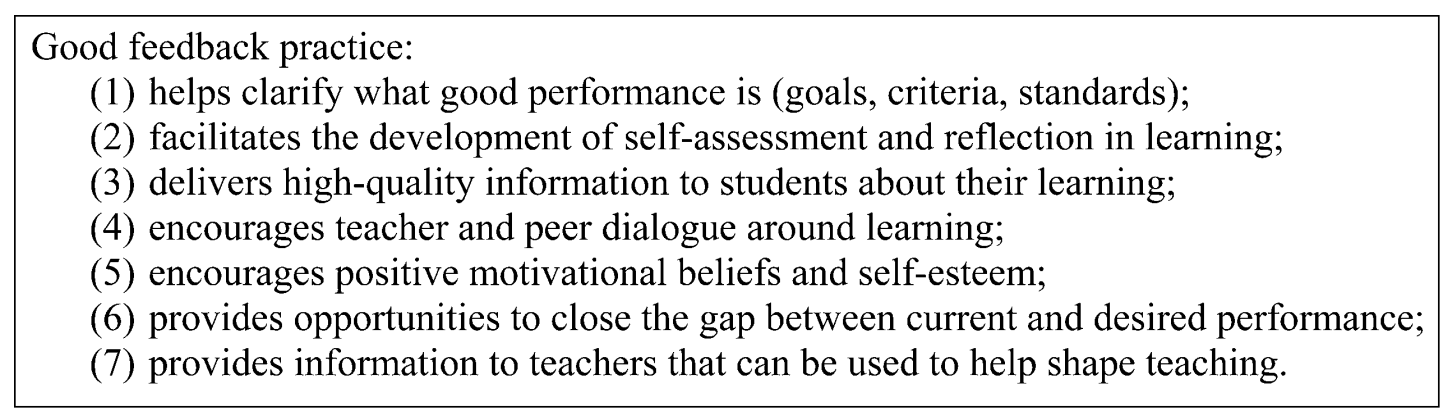
\includegraphics[width=0.8\textwidth]{multipleChoice.png}
    \caption{Seven principles of good feedback practice \cite{nicol}.}
    \label{fig:sierra-practice}
\end{figure}

  Moreover, research on fixed mindset (I can't do X) versus growth mindset (I can't do X yet) talks about how mindset guides behaviour. In a math game with Dweck's research \cite{dweck-youtube} as a base, students were rewarded by the mentality of "Not yet" and effort versus getting a grade on existing knowledge. Regarding learning, those exposed to a growth mindset mentality, previously having a fixed mindset, got superior results, especially those students previously having difficulties with learning. Regarding motivation, Dweck's research showed that high achievers played to the end, but in the growth mindset version those still played to the end, but so many more lower and medium achievers also stayed until the end. \cite{dweck-youtube} \todo{Viktigt ta med detta i Resultat!}

  \subsubsection{Learning by Thinking: Reflection \& Retrieval Practice}

  Stefano \citep{stefano} suggests that that reflection has been an overlooked area of research for a long time. During the act of reflection, the student develops necessary skills and self-awareness to refine their own learning activities. His results suggests that reflection as an activity that can be more effective than additional learning. This surely applies to the teacher as well, Luckin says. \citep{luckin}

  Stefano found that individuals who are given time to reflect on a task, outperforms students who are given the same amount of time to practice with the same task. But, similar to deliberate practice, it is a desirable difficulty: individuals in the test themselves, had a tendency to believe that allocating time to practice on the task rather than reflecting on it would benefit them.

  %\subsubsection{Retrieval practice}

  When it comes to study technique, Bjork \citep{bjork} as well shows that retrieval from memory is more effective than people who repeat reading the same thing to remember: the more effective students, retrieves from memory.

  One way to use memory retrieval as a study technique, is to ask "What was in that article?", before checking the answer in the article (the flashcard principle). It is an example of memory retrieval that is extremely effective for learning, their research shows. There is a danger with multiple-choice questions, that the student is given no time to reflect on the question and their prior knowledge, before evaluating the alternatives.



%\subsubsection{Not forgetting}

%UCLA Bjork's Learning and Forgetting Lab researches how people forget, and how to design so that people do not forget.

%\include{theory/learning/pedagogical-development/social_psychology}
